\documentclass{beamer}
\usepackage[polish]{babel}
\usepackage[utf8]{inputenc}

\usepackage{movie15}
\usepackage{hyperref}
\usepackage{wrapfig}


\usepackage{caption}

\usepackage{setspace}


%\usepackage{algorithm2e}
%\usepackage{algorithmic}
%\usepackage{float}
%\usepackage[noend]{algpseudocode}

\usepackage{algorithmic}

\usepackage[absolute,overlay]{textpos}

\usepackage[font=tiny]{subfig}
\usepackage{graphicx}



%https://gist.github.com/andrejbauer/ac361549ac2186be0cdb
\usepackage{pgfpages}
\usetheme{AGH}

\setbeameroption{hide notes} % Only slides
%\setbeameroption{show only notes} % Only notes
%\setbeameroption{show notes on second screen=right} % Both


% Give a slight yellow tint to the notes page
\setbeamertemplate{note page}{\pagecolor{yellow!5}\insertnote}\usepackage{palatino}

\title{Behawioralny algorytm koordynacji ruchu robotów mobilnych oparty na modelu postępowania przemieszczających się osób}
\author{mgr inż. Szymon Szomiński}

\supervisorPL{~dr~hab.~in\.z.~Aleksander~Byrski, prof. n.}
\supervisorPLsecond{~dr~in\.z.~Wojciech~Turek}
%\website{}
\date{6 grudzień 2018}

%TODO Numeracja do lewej 
%TODO numercja z pierszej strony ma zniknac

\begin{document}
	
{
\setbeamertemplate{footline}{}		
\titleframe[pl]
}

	

\begin{frame}
	\frametitle{Agenda}
	\tableofcontents
	
\note{
	
Dynamiczny rozwój  w dziedzinie mechaniki, elektroniki i informatyki przyczynił się do zintensyfikowania prac nad tworzeniem mobilnych platform robotowych. Już dziś roboty wyręczają człowieka w wykonywaniu różnorakich zadań takich jak: sprzątanie, poszukiwanie ludzi po trzęsieniu ziemi, inspekcja miejsc trudno dostępnych, patrolowanie i ochrona terenu  czy eksploracje przestrzeni kosmicznej. W związku z powyższym konieczne staje się poszukiwanie nowych metod koordynacji wielu niezalężnych jednostek mobilnych. 


}	
	
\end{frame}

\section{Inspiracje naturalne}
\begin{frame}
\frametitle{\secname}

%TODO Ruch na skrzyżowaniach

\begin{textblock*}{6.5cm}(1cm,2.5cm) % {block width} (coords)
\begin{itemize}
	\item Unikanie konfliktów z ,,większym'' lub ,,silniejszym'' osobnikiem.
	\item Chęć grupowania.
	\item Hierarchia społeczna.	
	\item Zasady ruchu drogowego.
\end{itemize}
\end{textblock*}

\begin{textblock*}{5cm}(7.7cm,1.8cm) % {block width} (coords)
	\includegraphics[page=3,width=5cm]{img/Rysunki.pdf}
	\tiny{Źródło: East News/Glow Images}
\end{textblock*}

\begin{textblock*}{6cm}(1.5cm,5.5cm) % {block width} (coords)
	\includegraphics[page=4,width=6cm]{img/Rysunki.pdf}
	\tiny{Źródło: www.itprotoday.com}
\end{textblock*}

\begin{textblock*}{5cm}(7.7cm,5cm) % {block width} (coords)
	\includegraphics[page=5,width=5cm]{img/Rysunki.pdf}
\end{textblock*}

\note{Zarówno wśród zwierząt jak i ludzi obserwuje się podświadome unikanie konfliktów z ,,większymi'' lub ,,silniejszymi'' osobnikami. Osobniki czujące się pewniej zakładają, iż ,,mniejsi'' ustąpią im miejsca. 
	
W środowisku zwierząt, obserwuje się podświadomą chęć grupowania osobników w ławice, watahy czy hordy. W większych skupiskach zwierzęta zwiększają swoje szanse na przetrwanie, w początkowym okresie swojego życia.

Obserwacje tę skłoniły do stworzenia algorytmu bazującego na zjawisku respektu który modelowany jest za pomocą wzoru.

Ze zbioru robotów $ Z $ ...
Znajdujące się w pewnej odległości od siebie roboty Dmax stają się członkami grupy gdy ich 

	
Wśród ludzi obserwuje się również podświadomą chęć grupowania, wynikająca z pierwotnych instynktów, ale również przekazywania zdobytej wiedzy następnym pokoleniom. Hierarchia społeczna odnoszona jest zwykle do społeczności ludzkiej, w której niektóre z osobników znajdują się wyżej w stosunku do innych. Taki podział może mieć różne podłoża, w zależności od grupy. Najbardziej naturalny dla ludzi wynika, z wieku osobników czy ich płci. Młodsze osobniki darzą należnym im, szacunkiem osobniki starsze. Organizacja grupy społecznej widoczna jest najlepiej, w relacjach zawodowych. Osoby zajmujące wysokie stanowiska kierowniczych, obdarzane są przez osoby na niższych stanowiskach respektem. Respekt nie wynika tylko z pozycji, jaką zajmuje dany osobnik w hierarchii. Zjawisko to jest znacznie bardziej szerokie i właśnie ono, dzięki temu zainspirowało autorów do stworzenia algorytmu koordynacji ruchu robotów mobilnych.}

\end{frame}

\section{Zjawisko respektu}
\begin{frame}
\frametitle{\secname}

\begin{textblock*}{5cm}(0.3\linewidth,2cm) % {block width} (coords)
	\begin{equation*}
	k_j = \sum_{i \in Z}  \left(   \frac{D_{max} - d_{ij}}{D_{max}} ~ \cdot ~ cos(\phi_{ij}) ~ \cdot f_i \right)
	\end{equation*}
\end{textblock*}

\begin{textblock*}{5cm}(7cm,4.2cm) % {block width} (coords)
	\scriptsize{
		\begin{tabular}{lp{0.85\textwidth}}
			$ k_j $       	& Współczynnik respektu dla \textit{j--tego} robota. \\
			$ d_{ij} $    	& Odległość pomiędzy robotem \textit{i--tym} oraz \textit{j-tym}. \\
			$ \phi_{ij} $ 	& Kąt skierowany pomiędzy robotem \textit{i--tym} oraz \textit{j--tym}. \\
			$ f_i $ 		& Bazowy współczynnik respektu dla \textit{i-tego} robota. Znany wszystkim uczestnikom ruchu oraz stały w czasie wyznaczania trajektorii ruchu przez wszystkich robotów. \\
			$ D_{max} $ 	& Zasięg.  \\
			$ Z $ 			& Zbiór robotów znajdujących się w zasięgu $ D_{max} $ \textit{j-tego} robota.	
	\end{tabular}}
\end{textblock*}

\begin{textblock*}{6cm}(1cm,5cm) % {block width} (coords)
	\includegraphics[page=5,width=6cm]{img/hybrid_algorithm.pdf}
\end{textblock*}

\note{Wprowadzono sztuczną funkcję używaną do określenia, który robot posiada większy stopień respektu. Roboty nie negocjują ani nie wymieniają się żadnymi informacjami potrzebnymi do wyliczenia współczynnika. Żadnemu z robotów nie przypisuje się również odgórnie konkretnego stopnia respektu. Każdy z robotów autonomicznie, w sposób całkowicie zdecentralizowany wylicza wartość \textit{współczynnika respektu}, bazując wyłączenie na obserwacji innych uczestników ruchu. \textit{Współczynnik respektu} reprezentowany jest przez pojedynczą wartość zmiennoprzecinkową $ k_j $ obliczaną według wzoru:}

\note{W przestrzeni w której nie wystębuje duża ilość przeszkud statycznych oraz roboty moga sfobodnie się przemiszczać zjawiko raspketu może być z powodzeniem stosowane. Stworzono dwa algorytmu bazające na Zjawisku Respektu: R oraz R+}

\note{Bazując na \textit{zjawisku respektu} stworzono dwie metody, których działania wykorzystują jego właściwości.}

\end{frame}	

\subsection*{Pseudo-kod implementacja algorytmu Respect (R)}
\begin{frame}
\frametitle{\subsecname}
\scriptsize{		
	\begin{algorithmic}[1]	
		\REPEAT
		
		\STATE $ goal_{i} = \Upsilon(pos_{i}) $
		
		\STATE $ Z \gets RobotsWithFixedDistance(pos_{i},Rob) $
		\STATE $ k_{i} \gets k(pos_{i},Z) $
		
		\STATE  $ robotsWithLowerRespectTooClose \gets GetLowerRespectRobots(k_{i},Z) $
		
		\STATE  $ robotsWithHigherRespect \gets GetHigherRespectRobots(k_{i},Z) $
		
		\IF{$ robotsWithLowerRespectTooClose.Count > 0 $}
		\STATE	$ \kappa(i, robotsWithLowerRespectTooClose) $ 
		\ELSE			
		\IF{$ robotsWithHigherRespect.Count > 0 $}
		\STATE $ \kappa(i, robotsWithHigherRespect) $
		\ELSE	
		\STATE $ \kappa(i, r_{i}) $ 
		\ENDIF
		\ENDIF
		\UNTIL{$ goal_{i} \neq \varnothing $}	
\end{algorithmic}}

\note{Pierwszy z algorytmów został nazwany Respect (R). Listing  przedstawia implementację w pseudo-kodzie poszczególnych kroków działania algorytmu R.}

\note{Algorytm \textit{R} pobiera lokalizacje uczestników ruchu (linia: 4), wyznacza swój \textit{współczynnik respektu} zgodnie ze wzorem \ref{eq:fearFactor} (linia: 5). W kolejnym etapie metoda sprawdza czy trajektoria robota koliduje z trajektoriami pozostałych uczestników ruchu, czy też nie (linie: 6-7). Jeżeli trasa pokrywa się z trasą innego robota, w celu wyznaczenia pierwszeństwa dokonywane jest porównanie obliczonych \textit{współczynników respektu}. Gdy \textit{współczynnik respektu} jest mniejszy  niż \textit{współczynnik respektu} robota kolidującego, robot zmuszony jest do ustąpienia mu pierwszeństwa i wyznaczenia nowej trasy (linia: 12). Jeżeli trajektoria robota nie koliduje z robotem o większym \textit{współczynniku respektu}, robot wyznacza najkrótsza trasę do celu wykorzystując algorytm \cite{TurekCetnarowiczZaborowski2011} (linia: 14). Do wyznaczenia nowej bezkolizyjnej ścieżki w~algorytmie \textit{R} brane są pod uwagę wyłącznie te roboty, których obliczone \textit{współczynniki respektu} są większe od \textit{współczynnika respektu} bieżącego robota (linia: 12). Algorytm zakłada, iż roboty o mniejszym \textit{współczynniku respektu} ustąpią pierwszeństwa robotowi o wyższym \textit{współczynniku respektu}. Procedura powtarzana jest dopóty, dopóki wszystkie cele robota nie zostaną osiągnięte (linia: 15).}
\end{frame}

\subsection*{Pseudo-kod implementacja algorytmu Respect+ (R+)}
\begin{frame}
\frametitle{\subsecname}
\scriptsize{		
\begin{algorithmic}[1]	
	
	\REPEAT
	
	\STATE $ goal_{i} = \Upsilon(pos_{i}) $
	
	\STATE $ Z \gets RobotsWithFixedDistance(pos_{i},Rob) $
	\STATE $ k_{i} \gets k(pos_{i},Z) $
	
	\STATE  $ robotsWithLowerRespectTooClose \gets GetLowerRespectRobots(k_{i},Z) $
	
	\STATE  $ robotsWithHigherRespect \gets GetHigherRespectRobots(k_{i},Z) $
	
	\STATE  $ allCollisionRobots \gets GetAllCollisionRobots(k_{i},Z) $
	
	\IF{$ robotsWithLowerRespectTooClose.Count > 0 $}
	\STATE	$ \kappa(i, robotsWithLowerRespectTooClose) $ 
	\ELSE			
	\IF{$ robotsWithHigherRespect.Count > 0 $}
	\STATE $ \kappa(i, robotsWithHigherRespect) $
	\ELSE	
	\STATE $ \kappa(i, allCollisionRobots) $ 
	\ENDIF
	\ENDIF
	\UNTIL{$ goal_{i} \neq \varnothing $}
\end{algorithmic}}

\note{Listing przedstawia implementację w pseudo-kodzie poszczególnych kroków działania algorytmu Respect+ (R+)}

\note{Metoda Respect+ (R+), podobnie jak metoda Respect (R), pobiera lokalizacje robotów (linia: 4), oblicza \textit{współczynnik respektu} (linia: 5), lecz wyznaczanie trajektorii ruchu przebiega w nieco odmienny sposób. W algorytmie \textit{R+} robot, który nie musi ustąpić pierwszeństwa ruchu przejazdu innym robotom, stara się pokonać trasę do celu bez modyfikowania swojej trajektorii. Jeżeli jednak nie jest możliwy bezkolizyjny ruch, dokonywana jest korekcja trajektorii uwzględniająca bieżącą pozycję innych uczestników ruchu (linia: 15). Robot, którego obliczony współczynnik respektu jest mniejszy od współczynników respektu pozostałych uczestników ruchu, zobligowany jest do zmiany swojej trasy w celu ustąpienia pierwszeństwa (linia: 13).}

\end{frame}

\section{Zasada priorytetyzowania wychodzących}
\begin{frame}
\frametitle{\secname}

\begin{textblock*}{5cm}(0.3\linewidth,1.5cm) % {block width} (coords)
	\begin{equation*}
	p_j = 1 + \psi\left(d_{jl}\right) * \lambda\left(\alpha_j,\gamma_l\right) * \tau 
	\end{equation*}
\end{textblock*}

\begin{textblock*}{5cm}(0.1\linewidth,2.5cm) % {block width} (coords)
	\footnotesize{
		\begin{equation*}
		\psi\left(d_{jl}\right) = \left\{\begin{array}{ll}
		\frac{R_{l} - d_{jl}}{R_{l}} \mbox{ dla } d_{jl} \le R_{l} \\
		0 \mbox{ w innym przypadku }        
		\cr
		\end{array}\right.
		\end{equation*}
	}
\end{textblock*}

\begin{textblock*}{5cm}(0.6\linewidth,2.5cm) % {block width} (coords)
	\footnotesize{
		\begin{equation*}
		\lambda\left(\alpha_j,\gamma_l\right) = \left\{\begin{array}{ll}
		1  \mbox{ dla } - \frac{\pi}{2} \leq \alpha_j - \gamma_l \leq \frac{\pi}{2} \\
		0  \mbox{ w innym przypadku }
		\cr
		\end{array}\right.
		\end{equation*}	
	}
\end{textblock*}

\begin{textblock*}{4.8cm}(7cm,3.8cm) % {block width} (coords)
	\scriptsize{
		\begin{tabular}{lp{0.85\textwidth}}
			$ p_j $ 						& Czynnik przejścia przez drzwi dla  \textit{j-tego} robota.\\
			$ \psi\left(d_{jl}\right) $ 	& Funkcja określająca w jakim stopniu robot jest w zasięgu działania drzwi.\\
			$ \lambda(\alpha_j,\gamma_l) $ 	& Funkcja, która decyduje czy robot \textit{j-ty} wchodzi do pomieszczenia, czy wychodzi z niego.\\
			$ \tau \in \mathbb{R}_{+} $ 	& Współczynnik definiujący wpływ czynnika przejścia na pierwszeństwo.\\
			$ d_{jl} $ 						& Dystans pomiędzy robotem \textit{j-tym} oraz środkiem \textit{l-tego} przejścia.\\
			$ l $ 							& Identyfikator przejścia (drzwi). \\
			$ \gamma_l $ 					& Kąt skierowania wersora wskazującego kierunek ,,wychodzenia'' przez drzwi.
		\end{tabular}
	}
\end{textblock*}

\begin{textblock*}{6cm}(1cm,5cm) % {block width} (coords)
	\includegraphics[page=6,width=6cm]{img/hybrid_algorithm.pdf}
\end{textblock*}

%\note{Gdzie:
%	pj       - Czynnik przejścia przez drzwi dla robota  j .
%	ψ(djl)  - Funkcja określająca, w jakim stopniu robot jest w zasięgu działania drzwi.
%	λ(αj,γl) - Funkcja która decyduje, czy robot j wchodzi do pomieszczenia czy wychodzi z niego.
%	τ ϵ R+    - Współczynnik definiujący wpływ czynnika przejścia na pierwszeństwo. W eksperymentach przyjęliśmy wartość  τ = 1, ale możliwe jest dynamiczne określanie tego współczynnika na przykład na podstawie stosunku zagęszczeń robotów w sąsiadujących pomieszczeniach.
%	djl  - Dystans pomiędzy robotem  j  oraz środkiem przejścia (drzwiami)  l  (można zmienić na odległość od odcinka stanowiącego drzwi).
%	l - Identyfikator drzwi. Lokalizacja drzwi, ich szerokość oraz kierunek otwarcia zdefiniowane zostały w pliku mapy labiryntu i są dostępne dla każdego z robotów.
%	γl  - kąt prostopadły do odcinka reprezentującego drzwi, wskazujący kierunek ,,wychodzenia'' przez drzwi. 
%	Rl  - Maksymalny zasięg działania drzwi l.}

\end{frame}

\section*{Integracja zjawiska respektu z czynnikiem przejścia przez drzwi}
\begin{frame}
\frametitle{\secname}

\begin{textblock*}{5cm}(0.4\linewidth,2cm) % {block width} (coords)
	\begin{equation*}
	KP_j = k_j * p_j
	\end{equation*}
\end{textblock*}

\begin{textblock*}{6cm}(0.25\linewidth,3cm) % {block width} (coords)
	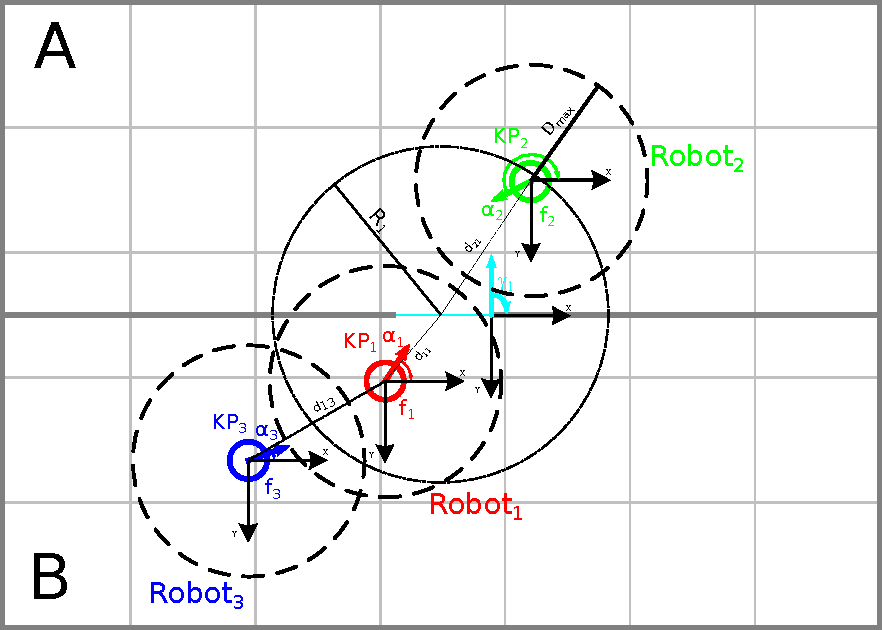
\includegraphics[page=1,width=8cm]{img/AlgorytmPrzejsciaPrzezDrzwi.pdf}
\end{textblock*}

\note{W oparciu o rozrzeszoną metodę Passage Factor (PF) oraz jego odmianę PF+. Algorytm PF wykorzystuje właściwości algorytmu \textit{R} uzupełnionego o zasadę priorytetyzowania robotów w trakcie opuszczania pomieszczenia.}

\end{frame}

\subsection*{Pseudo-kod implementacja algorytmu Passage Factor (PF)}
\begin{frame}
\frametitle{\subsecname}
\scriptsize{		
	\begin{algorithmic}[1]
		
		\REPEAT
		
		\STATE $ goal_{i} = \Upsilon(pos_{i}) $
		
		\STATE $ Z \gets RobotsWithFixedDistance(pos_{i},Rob) $
		\STATE $ door_{l} \gets GetDoorFromMap(l) $
		\STATE $ kp_{i} \gets KP(pos_{i}, Z, door_{l}) $
		
		\STATE  $ robotsWithLowerRespectTooClose \gets GetLowerRespectRobots(kp_{i},Z) $
		
		\STATE  $ robotsWithHigherRespect \gets GetHigherRespectRobots(kp_{i},Z) $
		
		\IF{$ robotsWithLowerRespectTooClose.Count > 0 $}
		\STATE	$ \kappa(i, robotsWithLowerRespectTooClose) $ 
		\ELSE			
		\IF{$ robotsWithHigherRespect.Count > 0 $}
		\STATE $ \kappa(i, robotsWithHigherRespect) $
		\ELSE	
		\STATE $ \kappa(i, r_{i}) $ 
		\ENDIF
		\ENDIF
		\UNTIL{$ goal_{i} \neq \varnothing $}
		
\end{algorithmic}}
\end{frame}		


\subsection*{Pseudo-kod implementacja algorytmu  Passage Factor (PF+)}
\begin{frame}
\frametitle{\subsecname}
\scriptsize{		
\begin{algorithmic}[1]
	\REPEAT
	
	\STATE $ goal_{i} = \Upsilon(pos_{i}) $
	
	\STATE $ Z \gets RobotsWithFixedDistance(pos_{i},Rob) $
	
	\STATE $ door_{l} \gets GetDoorFromMap(l) $
	\STATE $ kp_{i} \gets KP(pos_{i}, Z, door_{l}) $
	
	\STATE  $ robotsWithLowerRespectTooClose \gets GetLowerRespectRobots(kp_{i},Z) $
	
	\STATE  $ robotsWithHigherRespect \gets GetHigherRespectRobots(kp_{i},Z) $
	
	\STATE  $ allCollisionRobots \gets GetAllCollisionRobots(kp_{i},Z) $
	
	\IF{$ robotsWithLowerRespectTooClose.Count > 0 $}
	\STATE	$ \kappa(i, robotsWithLowerRespectTooClose) $ 
	\ELSE			
	\IF{$ robotsWithHigherRespect.Count > 0 $}
	\STATE $ \kappa(i, robotsWithHigherRespect) $
	\ELSE	
	\STATE $ \kappa(i, allCollisionRobots) $ 
	\ENDIF
	\ENDIF
	\UNTIL{$ goal_{i} \neq \varnothing $}	
	
\end{algorithmic}}
\end{frame}		

\section{Zasada prawej dłoni}
\begin{frame}
\frametitle{\secname}
\framesubtitle{Pseudo-kod implementacja algorytmu  Priority to the Right (PR)}
\scriptsize{		
	\begin{algorithmic}[1]
		
		\REPEAT
		
		\STATE $ goal_{i} = \Upsilon(pos_{i}) $
		
		\STATE $ Z \gets RobotsWithFixedDistance(pos_{i},Rob) $
		
		\STATE $ robotsOnTheRightSide \gets GetRobotOnTheRightSide(pos_{i}) $
		
		\IF{$ robotsOnTheRightSide.Count > 0 $}
		\STATE	$ \kappa(i, robotsOnTheRightSide) $ 
		\ELSE			
		\STATE $ \kappa(i, r_{i}) $ 
		\ENDIF
		
		\UNTIL{$ goal_{i} \neq \varnothing $}
		
\end{algorithmic}}

\note{Inspiracją do za-modelowania \textit{zasada prawej dłoni} została zapożyczona z prawa ruchu drogowego oraz reguł poruszania się obowiązujących na wodzie. W środowisku, w~którym poruszają się roboty rzadko spotyka się wyznaczone pasy ruchu.
	
W stworzonej metodzie pierwszeństwo poruszania się mają roboty nadjeżdżające z~prawej strony. Na listingu zaprezentowano kolejne etapy działania algorytmu PR.}

\note{Jeżeli robot wykryje robota nadjeżdżającego z prawej strony, to w zaistniałej sytuacji zobligowany jest do ustąpienia mu pierwszeństwa. Robot zmienia swoją dotychczasową trajektorię ruchu starając się ominąć robota zbliżającego się z prawej strony (linia: 7). Gdy roboty wzajemnie się wyminą, robot wyznacza trajektorię do celu (linia: 9), aby powrócić do wykonywania powierzonego zadania.}

\end{frame}		


\section{Przypadki testowe}
\begin{frame}
\frametitle{\secname}

\begin{itemize}
	\item Otwarta przestrzeń.
	\item Przejście przez drzwi.	
	\item Wąski korytarz.
	\item Skrzyżowanie równorzędne.
	\item Skrzyżowanie typu 8.
	\item Mijanka.	
\end{itemize}

\begin{textblock*}{8cm}(6.6cm,1.85cm) % {block width} (coords)
	
	\includegraphics[page=5,width=3cm]{img/experimental_results.pdf}
	\includegraphics[page=18,width=3cm]{img/experimental_results.pdf}
	
	\includegraphics[page=6,width=3cm]{img/experimental_results.pdf}	
	\includegraphics[page=8,width=3cm]{img/experimental_results.pdf}
	
	\includegraphics[page=9,width=3cm]{img/experimental_results.pdf}
	\includegraphics[page=10,width=3cm]{img/experimental_results.pdf}
	
\end{textblock*}

\begin{textblock*}{5cm}(1.2cm,7.8cm) % {block width} (coords)
	\includegraphics[page=11,width=5cm]{img/experimental_results.pdf}	
\end{textblock*}

\note{
	
	Ustawienie prostopadłe: 
	1-1 do 10-10 robotów
	
	Skos:
	4 roboty 
	Zadanie 1 polegało na przejechaniu po skosie do punktu leżącego po przekątnej
	Zadanie 2 polegało na przejechaniu po skosie do punktu leżącego po przekątnej oraz powrót do punktu startu
	
	Przejście przez drzwi:
	1-H1 do 10-H10
	Oraz 
	H1-1 do H1-1
	H – w którym pomieszczeniu roboty miały wyższy bazowy współczynnik respektu.
	
	Wąski korytarz:
	1-1 do 10-10
	
	Skrzyżowania:
	Dwa roboty
	
	Dwa roboty
	Cztery roboty
	
	Mijanka:
	1-H1
	H1-1}

\end{frame}


\section{Wyniki eksperymentów symulacyjnych}
\begin{frame}
\frametitle{\secname}
\framesubtitle{Otwarta przestrzeń ustawienie prostopadłe}
	\begin{figure}[ht] % h:here; t:top; b:bottom; p:page; default:ht
		\centering
			\captionsetup[subfigure]{labelformat=empty}
			\centering
			\subfloat[][1-2]
			{
				\includegraphics[page = 2, width=0.49\textwidth]{img/Simulation_Open_space.pdf}
			}
			\subfloat[][10-9]
			{
				\includegraphics[page = 99, width=0.49\textwidth]{img/Simulation_Open_space.pdf}
			}
\end{figure}

\note{
\begin{itemize}
	\item Dla ustawienie 1-2 najlepszy łączny czas przejazdu robotów uzyskała algorytm PR. Jako drugi poradził sobie z zadaniem algorytm RVO. Algorytmy R+ oraz R osiągnęły podobne rezultaty.

	\item Przy większej liczbie robotów sytuacja znacząco się zmienia. Algorytm R osiągał najlepszy czas jako drugi algorytm R+. Trzecie miejsce to algorytm RVO zaś najgorzej poradziła sobie metoda PR.
\end{itemize}
}

\end{frame}

\section*{Wyniki eksperymentów symulacyjnych -- materiał wideo}
\begin{frame}
\frametitle{\secname}
\framesubtitle{Otwarta przestrzeń ustawienie prostopadłe 1-2}


\begin{center}
	\href{run:RobotSimulationOpenSpace.avi}{Materiał wideo}
\end{center}

%\begin{center}
%	 \includemovie[poster]{300pt}{200pt}{./mov/RobotSimulationOpenSpace.swf} 
%\end{center}

%\begin{figure}
%	\includemovie[autoplay,repeat]{0.24\paperwidth}{4cm}{mov/RobotSimulationOpenSpace.avi}
%	\caption*{Otwarta przestrzeń ustawienie prostopadłe 1-2}
%\end{figure}


\end{frame}


\section*{Wyniki eksperymentów symulacyjnych}
\begin{frame}
\frametitle{\secname}
\framesubtitle{Przejście przez drzwi}
\begin{figure}[ht] % h:here; t:top; b:bottom; p:page; default:ht
		\captionsetup[subfigure]{labelformat=empty}
		\centering
		\subfloat[][1-H2]
		{
			\includegraphics[page = 2, width=0.49\textwidth]{img/Simulation_Passage_through_the_door.pdf}
		}
		\subfloat[][9-H8]
		{
			\includegraphics[page = 88, width=0.49\textwidth]{img/Simulation_Passage_through_the_door.pdf}
		}
\end{figure}

\note{

\begin{itemize}
	\item Metoda RVO oraz PR nie poradziły sobie zarówno w ustawieniu 1-H2 oraz 9-H8. Roboty wzajemnie zakleszczyły się w przed przejściem.
	
	\item W obu ustawieniach wyraźnie zaznacza się trend iż metoda PF, PF+ jest nieco lepsza niż metoda R, R+
	
	\item Algorytmy R+ oraz PF+ osiągnęły gorsze wyniki niż metody R oraz R+
\end{itemize}

Litera H – oznaczona w którym pomieszczeniu roboty miały wyższe bazowy współczynnik respektu.

}

\end{frame}

\section*{Wyniki eksperymentów symulacyjnych}
\begin{frame}
\frametitle{\secname}
\framesubtitle{Wąski korytarz}

\begin{figure}[ht] % h:here; t:top; b:bottom; p:page; default:ht
	\captionsetup[subfigure]{labelformat=empty}
	\centering
	\subfloat[][8-3]
	{
		\includegraphics[page = 73, width=0.6\textwidth]{img/Simulation_A_narrow_corridor.pdf}
	}
\end{figure}

\note{
	
	\begin{itemize}
		\item Również i w wąskim korytarzu metody RVO i PR nie poradziły sobie z zadaniem.
		\item Metoda R osiągnęła znacznie lepszy czas przejazdu niż metoda R+
	\end{itemize}
}

\end{frame}

\section*{Materiał wideo}
\begin{frame}
\frametitle{\secname}

Tu powstaje film 1min z eksperymentów symulacyjnych który będzie zawierał:

Otwarta przestrzeń ustawienie 1-2 algorytmy R RVO, PR R+
Przejście przez drzwi ustawienie 9-H8 algorytmy R PF RVO, PR R+, PF+
Wąski korytarz ustawienie 8-3 algorytmy R RVO, PR R+
\end{frame}


\section*{Eksperyment na rzeczywistych robotach}
\begin{frame}
\frametitle{\secname}

\begin{itemize}
	\item Obudowa A4WD1v2 Lynxmotion 22cm x 20cm x 6cm.
	\item Zasilanie dwie baterie litowo-polimerowe o nominalnym napięciu 14.8V i pojemności 5Ah.
	\item Sterowniki silników RoboClaw 2 x 15A firmy BasicMicro.
	\item Komputer sterujący PandaBoard ES:	
	\begin{itemize}
		\item dwurdzeniowy procesor Cortex-A9 OMAP4460 taktowany zegarem 1,2 GHz,
		\item RAM 1GB,
		\item Ethernet RJ45 100Mb,
		\item WiFi 802.11 b/g/n i Bluetooth 2.1,
		\item USB 2.0,
		\item I2C,
		\item SPI.
	\end{itemize}
	\item Skaner laserowy URG-04LX-UG01 firmy Hokuyo.	
\end{itemize}

\begin{textblock*}{4cm}(8.5cm,5.2cm) % {block width} (coords)
	\includegraphics[page=1,width=4cm]{img/Rysunki.pdf}
\end{textblock*}
\tiny{
	Open Source Hardware \\
	Strona projektu: \url{http://capo.iisg.agh.edu.pl/}}

\note{
W celu zweryfikowania poprawności działania algorytmów wykorzystano Czterokołową Autonomiczną Platformę Mobilną CAPO zbudowaną na AGH.

Platforma:

\begin{itemize}
	\item zasilana jest z dwóch baterii litowo-polimerowych, 
	\item napędzane jest przez 4 silniki kontrolowane przez dwa kontrolery RoboClaw 2 x 15A firmy BasicMicro,
	\item które kontroluje komputer sterujący PandaBoard ES.
\end{itemize}

Platforma może być dowolnie konfigurowana. Na rysunku widzimy robota CAPO z zaistalowanym skanerem laserowym firmy Hokuyo.

}
\end{frame}

\section{Wyniki eksperymentów z wykorzystaniem rzeczywistych robotów}
\begin{frame}
\frametitle{\secname}
\framesubtitle{Otwarta przestrzeń ustawienie prostopadłe}
\begin{figure}[ht] % h:here; t:top; b:bottom; p:page; default:ht
	\captionsetup[subfigure]{labelformat=empty}
	\centering
	\subfloat[][1-2]
	{
		\includegraphics[page = 2, width=0.6\textwidth]{img/Robots_Open_space.pdf}
	}
\end{figure}

\note{
\begin{itemize}
	\item Najlepiej z przejazdem poradziła sobie metoda PR.
	\item Metody R oraz R+ osiągnęły podobny rezultat.
	\item Metoda RVO zakończyła swoje działanie jako ostatnia.
\end{itemize}

}

\end{frame}

\section*{Wyniki eksperymentów z wykorzystaniem  rzeczywistych robotów}
\begin{frame}
\frametitle{\secname}
\framesubtitle{Przejście przez drzwi}
\begin{figure}[ht] % h:here; t:top; b:bottom; p:page; default:ht
	\captionsetup[subfigure]{labelformat=empty}
	\centering
	\subfloat[][1-H2]
	{
		\includegraphics[page = 2, width=0.6\textwidth]{img/Robots_Passage_through_the_door.pdf}
	}
\end{figure}

\note{
\begin{itemize}
	\item Metody RVO oraz PR ze względu na brak rezultatów w symulacji nie były uruchamiana na rzeczywistych robotach.
	\item Najlepiej poradziła sobie metoda PF+ oraz PF.
	\item Algorytm R osiągnął trzeci wynik.
	\item Najgorzej z zadaniem poradziła sobie metoda R+.
\end{itemize}
	
}

\end{frame}

\section*{Materiał wideo}
\begin{frame}
\frametitle{\secname}

Tu powstaje film 1min z eksperymentów na rzeczywistych robotach który będzie zawierał:

Otwarta przestrzeń ustawienie 1-2 algorytmy R RVO, PR R+
Przejście przez drzwi ustawienie 1-H2 dla algorytmów R, PF, R+ PF+
\end{frame}

\section{Wnioski i kierunki rozwoju}
\begin{frame}
\frametitle{\secname}

\begin{itemize}
	\item Prosty reaktywny zestaw reguł oparty na \textit{zjawisku respektu} sprawdza się w zatłoczonym środowisku, w którym bieżąca sytuacja zmienia się w sposób bardzo dynamiczny. 
	
	\item Wymuszenie ustępowania pierwszeństwa w oparciu o zasadę \textit{priorytetyzowania wychodzących} w wąskich przejściach zwiększa jego przepustowość. 
	
	\item \textit{Zasada prawej dłoni} nie radzi sobie dobrze przy ograniczonej ilości przestrzeni np. w \textit{wąskich korytarzach}.
	
	\item W bardziej skomplikowanych środowiskach, takich jak na przykład \textit{wąski korytarz} napotykamy na problem ,,przepychania'' się robotów.
	
\end{itemize}

\note{
\scriptsize		
		
\begin{itemize}
	\item Bazując wyłącznie na zdefiniowanych regułach behawioralnych oraz zasadzie pierwszeństwa jesteśmy w stanie zarządzać grupą robotów w mniej lub bardziej skomplikowanych środowiskach.
	
	\item Przykładem takim może być \textit{zasada prawej dłoni} bazująca na ustępowaniu pierwszeństwa jadącym z prawej strony i dobrze sprawdzająca się na skrzyżowaniach.  Metoda nie radzi sobie najlepiej przy ograniczonej ilości przestrzeni. W takiej sytuacji konieczne jest stosowanie innych metod zarządzania grupą robotów na przykład bazujących na zjawisku respektu.  Nie wszystkie wzorce zachowań dają dobre rezultaty w każdej sytuacji.
	
	\item  W środowiskach bardziej skomplikowanych, jak  \textit{przejście przez drzwi}, lepiej radzą sobie metody, które wymuszają przepustowość traktu komunikacyjnego.  Podnosząc priorytet robotom, które wychodzą z pomieszczenia udrażniamy przejście i tym samym zwiększamy jego przepustowość. 
	
	\item W bardzie skomplikowanych środowiskach koniecznej jest poszukiwanie innych metod koordynacji ruchu robotów.
	
	\item Analizując poszczególne eksperymenty można stwierdzić, iż postawiona teza pracy została udowodniona. Możliwe jest stworzenie zdecentralizowanego behawioralnego algorytmu sterowania ruchem robotów opartego na zachowaniu, inspirowanego postępowaniem przemieszczających się osób. Rozwiązanie to sprawdza się w środowiskach, w których konieczne jest skuteczne koordynowanie grupą robotów działających w dynamicznie zmieniającym się środowisku.
	
\end{itemize}	
}
\end{frame}
	


%\section*{Wnioski i kierunki rozwoju}
%\begin{frame}
%\frametitle{\secname}
%
%\begin{center}
%	\textbf{Możliwe jest stworzenie zdecentralizowanego behawioralnego algorytmu sterowania ruchem robotów opartego na zachowaniu, inspirowanego postępowaniem przemieszczających się osób.}
%\end{center}
%
%\note{
%	
%Analizując poszczególne eksperymenty można stwierdzić, iż postawiona teza pracy została udowodniona. Możliwe jest stworzenie zdecentralizowanego behawioralnego algorytmu sterowania ruchem robotów opartego na zachowaniu, inspirowanego postępowaniem przemieszczających się osób. Rozwiązanie to sprawdza się w środowiskach, w których konieczne jest skuteczne koordynowanie grupą robotów działających w dynamicznie zmieniającym się środowisku.
%}
%\end{frame}

\section*{Wnioski i kierunki rozwoju}
\begin{frame}
\frametitle{\secname}
\framesubtitle{Hybrydowy algorytm koordynacji ruchu robotów}

\begin{figure}[!hbp]
	\centering
	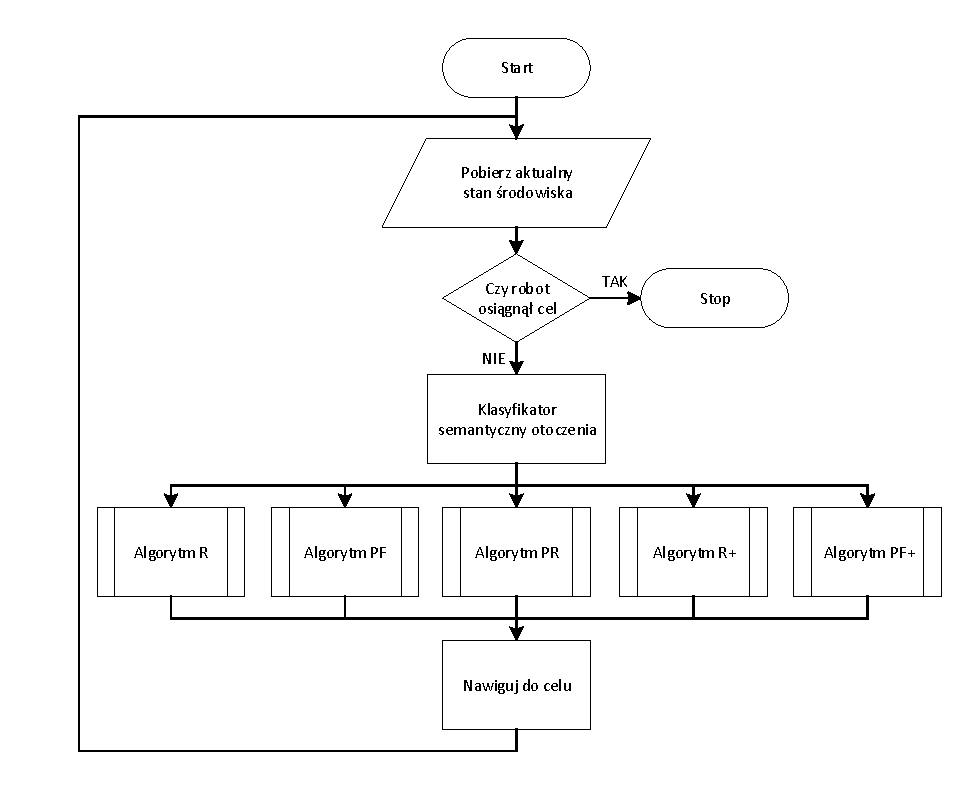
\includegraphics[page=1,width=0.85\textwidth]{img/hybrid_algorithm.pdf}
	
\end{figure} 
\note{
\begin{itemize}
	\item Oczywiście nie każda z metod jest na tyle uniwersalna, że można ją stosować we wszystkich przypadkach. Konieczne jest zatem dobieranie do danej sytuacji metod ją rozwiązujących. 

\item Połączenie kilku algorytmów, w jedno spójne rozwiązanie, umożliwi dostosowanie rozwiązania w zależności od bieżącej sytuacji. Taka zintegrowana metoda hybrydowa koordynacji ruchu pozwoli na optymalizację działania robota dla konkretnego przypadku. 
\end{itemize}

}
\end{frame}


{
\setbeamertemplate{footline}{}	
\begin{frame}
\begin{center}
	Dziękuje za uwagę
\end{center}
\end{frame}
}

\section*{1. pytanie prof. Stanisława Ambroszkiewicza}
\begin{frame}
\frametitle{\secname}
\framesubtitle{Czy przedstawiony  system wielo-robotowy jest rzeczywiście systemem rozproszonym?}

W literaturze znaleźć można różne definicje systemów rozproszonych (ang. distributed system). Tanenbaum w książce ,,Distributed systems: principles and paradigms''  definiują system rozproszony jako \textit{zbiór niezależnych urządzeń technicznych (komputerów) połączonych w jedną spójną logicznie całość}.

System rozproszony posiada następujące cechy:
\begin{itemize}
	\item przejrzystość (ang. transparency),
	\item dzielenie zasobów (ang. resource sharing),
	\item otwartość (ang. openness),
	\item współbieżność (ang. concurrency),
	\item skalowalność (ang. scalability),
	\item tolerowanie awarii (ang. fault tolerance).	
\end{itemize}

\note{

Komunikacja pomiędzy urządzeniami może być realizowana np. przez sieć komputerową lub magistrale komunikacyjne. Podstawową cechę, która charakteryzuje systemy rozproszone jest jego przejrzystość (ang. transparency) rozumiana poprzez sprawianie wrażania na użytkownikach, iż system stanowi pojedynczy i zintegrowany oraz spójny system.

Stworzony system wielo-robotowy posiada większość cech systemu rozproszonego. System cechuje współbieżność, gdyż posiada on zdolność do przetwarzania wielu zadań jednocześnie (np. analiza danych o lokalizacji robotów, wyznaczanie trajektorii ruchu). 

Podczas projektowania systemu wielo-robotowego jeden z kluczowych aspektów stanowiła tolerancja na awarię poszczególnych robotów. Stworzone rozwiązanie posiada mechanizmy umożliwiające reakcje (zatrzymania robota) w sytuacji, gdy może dojść do zakleszczenia czy spowodowanego awarią robota lub niemożnością wykonania powierzonego zadania (dojazd do punktu). System ma zagwarantować bezpieczną i skuteczną koordynację ruchu rozumianą ,,jako bezkolizyjne przemieszczanie się robotów'' (rozdział \ref{Section Teza pracy}). Zaś sama skuteczność ,,koordynacji rozumiana jest jako osiągniecie postawionego przed robotami celu (przemieszczenie się od punktu startu do punktu docelowego) oraz nie powodowanie zakleszczeń'' (rozdział \ref{Section Teza pracy}). Tak więc i ta cecha systemu może stanowić przesłankę do stwierdzenia, iż mamy do czynienia z systemem rozproszonym.

Patrząc na stworzony system wielo-robotowy możemy również dostrzec w nim cechę  przezroczystości systemu rozproszonego. Co prawda można zidentyfikować w nim poszczególne składowe, lecz patrząc całościowo na powierzone systemowi wielo-robotowemu zadania (dojazd do wyznaczonych lokalizacji) stworzone rozwiązanie dla obserwatora stanowi jedną spójną,  logiczną całość. 

Przytoczone cechy systemu rozproszonego zostały spełnione w skonstruowanym systemie wielorobotowym, dlatego zgodnie z moją najlepszą wiedzą można uznać ten system za rozproszony. Uwzględnienie pozostałych cech pozostaje oczywiście potencjalną kwestią dalszych prac.
}
\end{frame}

\section*{2. pytanie prof. Stanisława Ambroszkiewicza}
\begin{frame}
\frametitle{\secname}
\framesubtitle{Czy jest on otwarty, tj. czy nowe roboty i nowe powierzchnie do poruszania się dla tych robotów mogą być dodawane lub usuwane dynamicznie, a algorytmy nadal działają poprawnie?}

System posiada również cechę otwartości rozumianą jako możliwość rozbudowy systemu pod względem sprzętowym jak i programowym. Rozbudowa pod względem sprzętowym polega na dołączaniu do platformy CAPO nowych modułów poszerzających jego możliwości operacyjne. 
\newline
\newline
Wszystkie stworzone algorytmy są całkowicie bezstanowe, czyli nie są zależne od poprzedniego stanu systemu. Cecha ta umożliwia, po dostarczeniu algorytmowi danych zewnętrznych (informacji o lokalizacji i orientacji robotów), wyznaczenie w dowolnej iteracji sterowania dla poszczególnych robotów. Podobnie rzecz się ma z nowymi powierzchniami, które każdorazowo stanowią dane wejściowe dla algorytmów koordynacji. 

\note{

System posiada również cechę otwartości rozumianą jako możliwość rozbudowy systemu pod względem sprzętowym jak i programowym. Rozbudowa pod względem sprzętowym polega na dołączaniu do platformy CAPO nowych modułów poszerzających jego możliwości operacyjne. 

Aspekt programowy, rozumiany jako umożliwienie dynamicznego dołączania nowych robotów, został uwzględniony na etapie projektowania systemu wielo-robotowego.	Wszystkie stworzone algorytmy są całkowicie bezstanowe, czyli nie są zależne od poprzedniego stanu systemu. Cecha ta umożliwia, po dostarczeniu algorytmowi danych zewnętrznych (informacji o lokalizacji i orientacji robotów), wyznaczenie w dowolnej iteracji sterowania dla poszczególnych robotów. Podobnie rzecz się ma z nowymi powierzchniami, które każdorazowo stanowią dane wejściowe dla algorytmów koordynacji. 
	
Reasumując, ze względu na to, iż wszystkie algorytmy są całkowicie bezstanowe mogą działać w środowisku, które zmienia się w sposób całkowicie dynamiczny, czyniąc system otwartym i tym samym spełniając kolejną cechę ważną dla systemów rozproszonych.  

}

\end{frame}


\section*{3. pytanie prof. Stanisława Ambroszkiewicza}
\begin{frame}
\frametitle{\secname}
\framesubtitle{Jak jest faktyczna autonomia i niezależność robotów?}

Autonomia robotów (rozważana w kontekście sterownia i zarządzania grupą robotów mobilnych) umożliwia robotom niezależne wyznaczanie bezkolizyjnej trajektorii ruchu bez konieczności uzgadniania działań z innymi uczestnikami ruchu. Zadanie to jest realizowane w sposób całkowicie autonomiczny przez samego robota.  W oparciu o dane wejściowe (lokalizacji wraz z orientacją), robot podejmuje decyzję o wyborze trajektorii wyznaczonej w oparciu o jeden z algorytmów koordynacji.

\end{frame}


\section*{4. pytanie prof. Stanisława Ambroszkiewicza}
\begin{frame}
\frametitle{\secname}
\framesubtitle{\tiny{W eksperymentach roboty komunikują się z centralnym serwerem. A więc nie są one autonomiczne.  Czy nie prościej byłoby dodać prosty protokół komunikacyjny pomiędzy robotami, które siebie widzą, zachowując w ten sposób autonomiczność robotów?}}

Robot otrzymuje jedynie informacje o lokalizacji  oraz orientacji swojej oraz innych robotów z serwera lokalizacji. Procedura jest całkowicie niezależna od decyzji i operacji  wykonywanych przez roboty. Wszystkie roboty nasłuchują informacji wysyłanych z~serwera lokalizacji. Cały proces nie wymaga od nich zestawienia połączenia między sobą i jest niezależny od pozostałych działań poszczególnych uczestników ruchu. 
\newline
\newline
Wykorzystanie protokołu komunikacyjnego (nawet prostego) pomiędzy uczestnikami ruchu obarczone jest wieloma ograniczeniami oraz podatne jest na awaryjność. ,,Przy dużej ilości robotów, ograniczona przepustowość kanału komunikacyjnego może doprowadzić do spowolnienia lub zatrzymania pracy całego systemu'', lecz stanowi alternatywną wersję wzajemnego postrzegania się robotów.


\note{
Robot otrzymuje jedynie informacje o lokalizacji  oraz orientacji swojej oraz innych robotów z serwera lokalizacji. Procedura jest całkowicie niezależna od decyzji i operacji  wykonywanych przez roboty. Wszystkie roboty nasłuchują informacji wysyłanych z~serwera lokalizacji. Cały proces nie wymaga od nich zestawienia połączenia między sobą i jest niezależny od pozostałych działań poszczególnych uczestników ruchu. 

Bez znajomości lokalizacji poszczególnych robotów tworzony algorytm nie byłby w stanie funkcjonować. Problem wyznaczenia lokalizacji poszczególnych robotów jest koniecznym i złożonym procesem samym w sobie. Jednak niniejsza praca nie stanowi próby stworzenia nowego lub udoskonalenia już istniejącego sposobu lokalizacji robotów. Informacje o lokalizacji powinny być traktowane jedynie jako element techniczny systemu, innymi słowy: dane wejściowe dla algorytmów a nie element samych algorytmów.

Wykorzystanie protokołu komunikacyjnego (nawet prostego) pomiędzy uczestnikami ruchu obarczone jest wieloma ograniczeniami oraz podatne jest na awaryjność. ,,Przy dużej ilości robotów, ograniczona przepustowość kanału komunikacyjnego może doprowadzić do spowolnienia lub zatrzymania pracy całego systemu'' \cite{silver2005cooperative} rozdział \ref{Przegląd istniejących algorytmów koordynacji ruchu robotów mobilnych}, lecz stanowi alternatywną wersję wzajemnego postrzegania się robotów. Oprócz wykorzystania protokołu komunikacyjnego w celu wzajemnej identyfikacji oraz omijania robotów, konieczna jest jeszcze globalna lokalizacja robota na mapie, aby możliwe było wyznaczenie trajektorii robota do celu. Znajomość ,,globalnej'' lokalizacji umożliwia robotowi, w sposób całkowicie autonomiczny, wyznaczenie trajektorii ruchu w kierunku punktu docelowego. 

Innymi słowy, wprowadzenie protokołu komunikacyjnego tylko w celu ustalenia pozycji byłoby również elementem technicznym, komplikującym system natomiast nie wpływającym na działanie samych algorytmów.
}

\end{frame}
\section*{1. pytanie prof. Mariusza Zuberta}
\begin{frame}
\frametitle{\secname}
\framesubtitle{\fontsize{5}{0}\selectfont{Moje drobne zastrzeżenie budzi analiza poziomu ufności testów Dunna na podstawie uzyskanych wyników. Byłoby lepiej założyć poziom ufności i dla niego potwierdzić lub odrzucić hipotezę o statystycznej identyczności uzyskanych rozwiązań dla różnych algorytmów koordynujących ruch jednostek mobilnych.}}

\small
Rzeczywiście, proponowana przez Pana Profesora procedura jest standardowo stosowana przy testowaniu hipotez statystycznych i taką drogą niewątpliwie powinienem był postępować. Przekroczenie często przyjmowanej  wartości $\alpha=0.05$ jako prawdopodobieństwo, poniżej którego spełniona jest hipoteza zerowa wystąpiło w teście tylko w wybranych przypadkach, dlatego też zakładając potencjalne przeredagowanie treści, jestem przekonany że doszedłbym do podobnych wniosków, pomimo, jak Pan Profesor zauważył, zastosowania testu w niekonwencjonalny sposób, czyli wykryłbym identyczność rozkładów  następujących obserwacji (szczegółowe zestawienie przesłane w wersji elektronicznej) przy jednoczesnym potwierdzeniu istotności różnicy rozkładów opisujących pozostałe obserwacje. Oczywiście zastosuje się do uwagi Pana Profesora w kolejnych pracach, podczas analizy statystycznej wyników przeprowadzonych eksperymentów.

\note{
Rzeczywiście, proponowana przez Pana Profesora procedura jest standardowo stosowana przy testowaniu hipotez statystycznych i taką drogą niewątpliwie powinienem był postępować. Przekroczenie często przyjmowanej  wartości $\alpha=0.05$ jako prawdopodobieństwo, poniżej którego spełniona jest hipoteza zerowa wystąpiło w teście tylko w wybranych przypadkach, dlatego też zakładając potencjalne przeredagowanie treści, jestem przekonany że doszedłbym do podobnych wniosków, pomimo, jak Pan Profesor zauważył, zastosowania testu w niekonwencjonalny sposób, czyli wykryłbym identyczność rozkładów następujących obserwacji:

%\begin{itemize}
%	\item Eksperymenty symulacyjne:
%	\subitem \textit{otwarta przestrzeń} ustawienie: \textit{4-6} obserwacja (R -- R+): $4,985193 \cdot 10^{-1}$; (rozdział \ref{Podsumowanie_eksperymenty_symulacyjne}), 	
%	
%	\subitem \textit{otwarta przestrzeń okrąg} ustawienie: \textit{dwanaście robotów}, obserwacja (RVO -- R+): $3,36788 \cdot 10^{-1}$; (rozdział \ref{Wyniki_Otwarta_przestrzen_prostopadle_Ustawienie w okrąg}),
%	
%	\subitem \textit{przejście przez drzwi} ustawienia: \textit{1-H1} obserwacja (R -- PF): $0,5$; (rozdział \ref{Podsumowanie_eksperymenty_symulacyjne}),
%	
%	\subitem \textit{przejście przez drzwi} ustawienia: \textit{H1-4} obserwacja (R+ -- PF+): $4,43920 \cdot 10^{-1}$; (rozdział \ref{Wyniki_Przejscie_przez_drzwi}),
%	
%	\subitem \textit{przejście przez drzwi} ustawienie: \textit{H9-8} obserwacja (R+ -- PF+): $8,60042 \cdot 10^{-2}$; (rozdział \ref{Wyniki_Przejscie_przez_drzwi}),
%	
%	\subitem \textit{Skrzyżowanie typu 8} ustawienie: \textit{cztery roboty} obserwacja (R -- R+): $3,035915 \cdot 10^{-1}$; (rozdział \ref{Podsumowanie_eksperymenty_symulacyjne}), 
%	
%	
%	\item Eksperymenty z wykorzystanie rzeczywistych robotach:
%	
%	\subitem \textit{otwarta przestrzeń} ustawienie: \textit{1-2} obserwacja (R -- R+): $2,435655 \cdot 10^{-1}$; (rozdział \ref{Podsumowanie eksperymentów z wykorzystaniem rzeczywistych robotów}), 
%	
%	\subitem \textit{otwarta przestrzeń} ustawienie: \textit{skos [cztery roboty zadanie 2]} obserwacja (RVO -- R+): $4,363 \cdot 10^{-1}$; (rozdział \ref{Podsumowanie eksperymentów z wykorzystaniem rzeczywistych robotów}), 	
%	
%	\subitem \textit{przejście przez drzw} ustawienie: \textit{1-H1} obserwacja (PF -- PF+): $4,680237 \cdot 10^{-1}$; (rozdział \ref{Podsumowanie eksperymentów z wykorzystaniem rzeczywistych robotów}).	
%\end{itemize}

przy jednoczesnym potwierdzeniu istotności różnicy rozkładów opisujących pozostałe obserwacje.
Oczywiście zastosuje się do uwagi Pana Profesora w kolejnych pracach, podczas analizy statystycznej wyników przeprowadzonych eksperymentów. 

}
\end{frame}


\section*{2. pytanie prof. Mariusza Zuberta}
\begin{frame}
\frametitle{\secname}
\framesubtitle{\fontsize{4}{1}\selectfont{W pracy w zasadzie przedstawiono zaprezentowano algorytmy (R, R+ i PR) natomiast nie zostało dla mnie jasno przedstawiono czy w trakcie ,,pobieranie lokalizacji'' następuje synchronizacja tych algorytmów czy działają asynchronicznie. Jak to się ma do symulacji, która jest przeprowadzona z krokiem 0.2 sekundy. Dlatego proszę o wyjaśnienie jak jest różnica wzajemnej synchronizacji jednostek mobilnych podczas symulacji i rzeczywistych testów. }}

\scriptsize

W symulacji roboty są reprezentowane przez wątki uruchamiane niezależnie i nie synchronizowane (4 roboty, 4 wątki). Każdy z wątków pobiera informacje ze wspólnego wątku zwanego \textit{serwerem lokalizacji}, który w oparciu o wyznaczone przez wątek robota sterowanie oblicza jego nową pozycję, aby następnie rozesłać informacje do wszystkich pozostałych wątków. Pozbawiając synchronizacji poszczególne wątki można było, chociaż w niewielkim stopniu, odwzorować działanie wątków do działania rzeczywistych robotów. Wątki odświeżają lokalizację robotów co ok. 200 ms, a następnie przeliczane jest nowe sterowanie według jednego z~algorytmów koordynacji (R, R+, PF, PF+, PR).
\newline
\newline
W eksperymentach na rzeczywistych robotach proces uruchamiany był na robocie, który wykonywał stosowne obliczenia związane z algorytmem koordynacji oraz sterowaniem kołami robota. Pozycja robota w tym przypadku dostarczana była z zewnętrznego systemu przez \textit{serwer lokalizacji} (system z kamerą oparty na markerach Aruco). W eksperymentach wykorzystujących rzeczywiste roboty mobilne krok czasowy jest bardzo ciężki do oszacowania z uwagi na wywłaszczenia systemu operacyjnego działającego na robocie czy czas potrzebny na odbiór i przetworzenie wiadomości z danymi o lokalizacji dostarczanymi z \textit{serwera lokalizacji}. W zaistniałej sytuacji pominięto w pracy krok czasowy jaki robot potrzebuje do wykonania pojedynczego cyklu (pobranie lokalizacji,  wyznaczenie trajektorii, przemieszczenie się). 


\note{
W symulacji roboty są reprezentowane przez wątki uruchamiane niezależnie i nie synchronizowane (4 roboty, 4 wątki). Każdy z wątków pobiera informacje ze wspólnego wątku zwanego \textit{serwerem lokalizacji}, który w oparciu o wyznaczone przez wątek robota sterowanie oblicza jego nową pozycję, aby następnie rozesłać informacje do wszystkich pozostałych wątków. Pozbawiając synchronizacji poszczególne wątki można było, chociaż w niewielkim stopniu, odwzorować działanie wątków do działania rzeczywistych robotów. Założono, iż procedury obliczeń związanych ze zlokalizowaniem robotów (obliczenia lokalizacji) oraz obliczenia związane z algorytmami będą trwały ok. 200 ms i~stąd przyjęto tę wartość kroku czasowego symulacji. Wątki odświeżają lokalizację robotów co ok. 200 ms, a następnie przeliczane jest nowe sterowanie według jednego z~algorytmów koordynacji (R, R+, PF, PF+, PR).

W eksperymentach na rzeczywistych robotach proces uruchamiany był na robocie, który wykonywał stosowne obliczenia związane z algorytmem koordynacji oraz sterowaniem kołami robota. Pozycja robota w tym przypadku dostarczana była z zewnętrznego systemu przez \textit{serwer lokalizacji} (system z kamerą oparty na markerach Aruco). W eksperymentach wykorzystujących rzeczywiste roboty mobilne krok czasowy jest bardzo ciężki do oszacowania z uwagi na wywłaszczenia systemu operacyjnego działającego na robocie czy czas potrzebny na odbiór i przetworzenie wiadomości z danymi o lokalizacji dostarczanymi z \textit{serwera lokalizacji}. W zaistniałej sytuacji pominięto w pracy krok czasowy jaki robot potrzebuje do wykonania pojedynczego cyklu (pobranie lokalizacji,  wyznaczenie trajektorii, przemieszczenie się). 


}
\end{frame}


\section*{3. pytanie prof. Mariusza Zuberta}
\begin{frame}
\frametitle{\secname}
\framesubtitle{\tiny{Str. 67 ,,Roboty, których cele są zbieżne tworzą grupę,... Poprzez cele rozumieć należy wspólny kierunek ruchu...'' – proponuje sprecyzować, że chodzi o cele cząstkowe lub lokalne i kierunek ruchu w rozpatrywanej lokalizacji w aktualnej chwili czasowej. }}

Istotnie ta kwestia powinna być w pracy lepiej doprecyzowana, iż w każdej chwili czasowej roboty posiadają swoje cele cząstkowe zaś kierunek ruchu rozpatrywany jest w bieżącej chwili czasowej dla lokalizacji robotów. Dziękuję za zwrócenie uwagi na wspomnianą niejednoznaczność, którą można było różnie interpretować. 
\end{frame}

\section*{4. pytanie prof. Mariusza Zuberta}
\begin{frame}
\frametitle{\secname}
\framesubtitle{\fontsize{4.9}{1}\selectfont{Str. 67 ,,Pomiędzy poszczególnymi robotami występuje zależność osobnika obdarzonego większym respektem w stosunku do pozostałych uczestników ruchu'' – z punktu widzenia matematycznej relacji zapis jest poprawnym jednak z punktu widzenie ,,normalnego czytelnika'' w przyszłości proponuje rozważyć zamianę występujących podmiotów w przytoczonym zdaniu. }}

Bardzo dziękuję za tę sugestię. Z pewnością zgrabniej byłoby zmienić czy to szyk zdania lub rozwinąć szerzej wypowiedź tak, aby była bardziej przystępna oraz nie wzbudzała dyskomfortu w czytającym pracę.
\end{frame}

\section*{5. pytanie prof. Mariusza Zuberta}
\begin{frame}
\frametitle{\secname}
\framesubtitle{\fontsize{4.9}{1}\selectfont{Str. 68 ,,Współczynnik respektu reprezentowany jest przez pojedynczą liczbę rzeczywistą $ k_j $...'' – rozumiem o co chodzi autorowi rozprawy, jednak wydaje mi się bardziej zręczne zaznaczenie na początku pracy, że wszystkie wartości współczynników oraz zmiennych należą do zbioru liczb rzeczywistych i ewentualnie wskazanie zmiennych przyjmujących wartości dyskretne. }}
Tak, oczywiście zgadzam się z Pana Profesora opinią, iż należało na wstępie określić zbiorczo, które ze współczynników należą do zbioru liczb rzeczywistych, a które przyjmują wartości dyskretne. Tym samym, można było unikać dodatkowych wstawek w tekście między innymi takich jak ,,pojedyncza liczba rzeczywista'' itp.
\end{frame}

\section*{6. pytanie prof. Mariusza Zuberta}
\begin{frame}
\frametitle{\secname}
\framesubtitle{Strona 72-80, brak konsekwencji w formatowaniu nazw algorytmów: ,,PF'', ',,PF+'', ,,R'' i ,,R+''. Czasami nazwy są napisane kursywą a czasami czcionką bez kursywy. }
Bardzo dziękuję za to spostrzeżenie. Oczywiście jest to niedopatrzenie związane z~edytowaniem tekstu. W przyszłych pracach postaram się nie dopuścić do tego typu przeoczeń związanych z formatowaniem tekstu.
\end{frame}


\section*{7. pytanie prof. Mariusza Zuberta}
\begin{frame}
\frametitle{\secname}
\framesubtitle{\fontsize{5.6}{1}\selectfont{W pracy wielokrotnie występuje słowo ,,stworzyć''. W chwili obecnej odstępuje się od starych związków frazeologicznych tego słowa na rzecz bezpośredniego tłumaczenia angielskiego słowa ,,create''. Chciałbym jednak zasugerować przynajmniej próbę zastosowanie innego określenia w części wystąpień tego słowa. }}


Bardzo dziękuję za tę uwagę. Istotnie w pracy zbyt często użyto słowa ,,stworzyć'', które można było częściej substytuować, przykładowo słowem ,,utworzyć'' czy ,,opracować''. W kolejnych pracach postaram się używać synonimów  tego słowa i nie nadużywać go zbyt często w ramach akapitów, sąsiadujących stron tekstu oraz całych rozdziałów.
\end{frame}

\end{document}


%%Document
%\begin{figure}[htbp]
%	\centering
%	\includegraphics[page = 2, width=0.3\linewidth]{img/Simulation_Open_space.pdf}
%	\caption[short for lof]{long figure caption}
%	\label{fig:default}
%\end{figure}

%\begin{figure}[htbp] % h:here; t:top; b:bottom; p:page; default:ht
%	\centering
%	\subfloat[short for lof][long subfigure1 caption]{
%		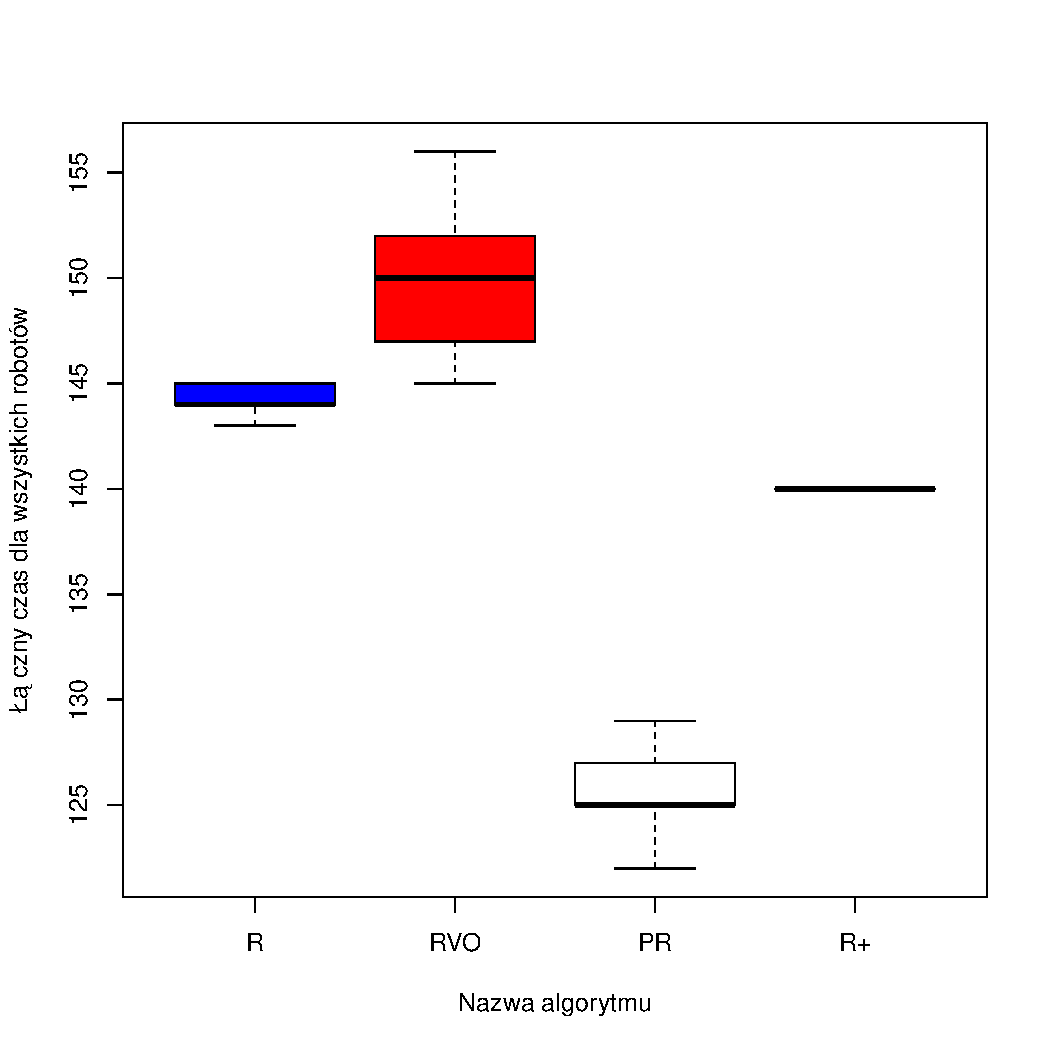
\includegraphics[width=0.3\linewidth]{img/Simulation_Open_space.pdf}
%		\label{subfig:fig1}
%	}
%	\subfloat[short for lof][long subfigure2 caption]{
%		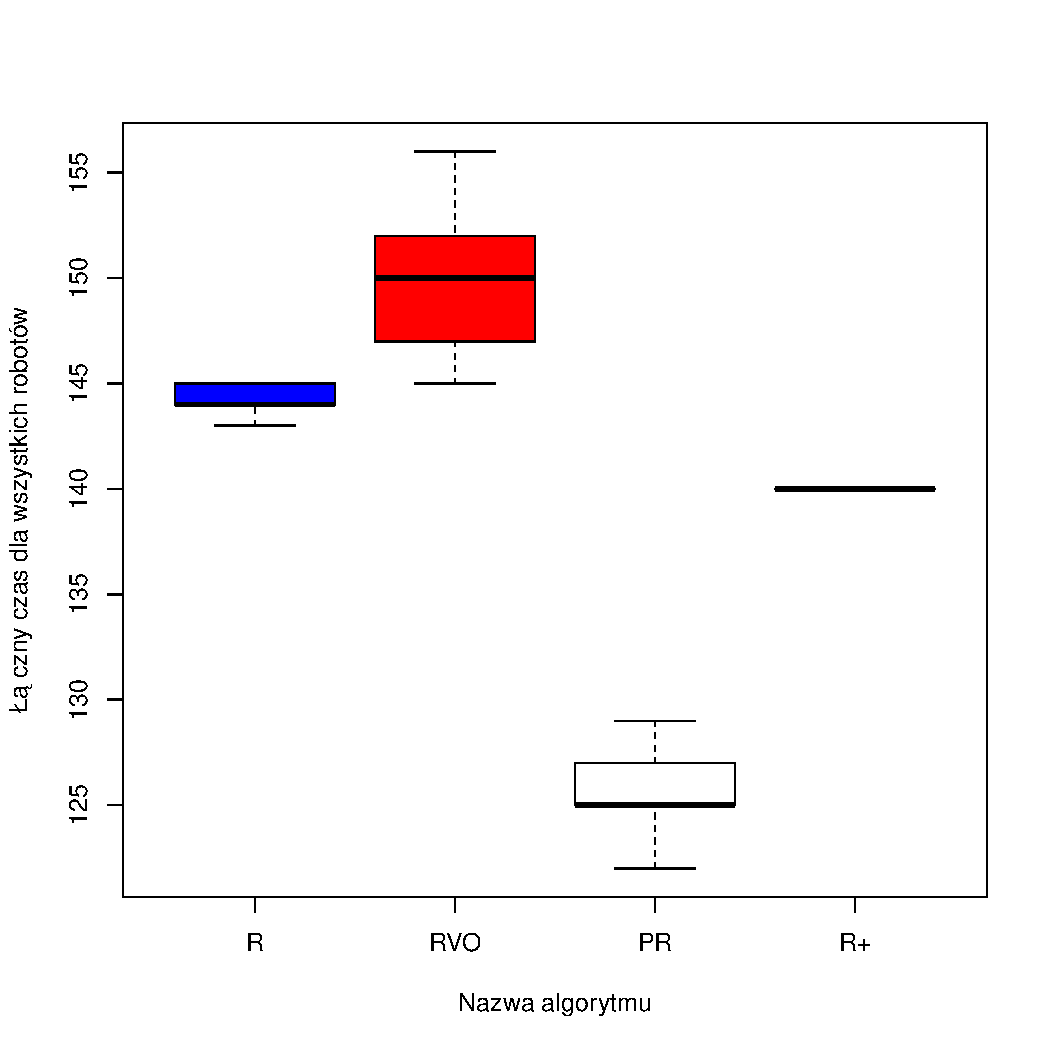
\includegraphics[width=0.3\linewidth]{img/Simulation_Open_space.pdf}
%		\label{subfig:fig2}
%	}
%	\caption[short for lof]{long figure caption}
%\end{figure}


%\begin{textblock*}{\textwidth}(0.0cm,0cm)
%	To jest tkest
%	\textblockcolour{red}
%\begin{figure}[!hb]
%	\includegraphics[page = 2, width=0.45\textwidth]{img/Simulation_Open_space.pdf}
%\end{figure}
%\end{textblock*}

%\begin{textblock*}{\paperwidth}(0.0cm,0cm)
%	\textblockcolour{red}
%\begin{figure}
%	\includemovie[autoplay,repeat]{0.24\paperwidth}{4cm}{mov/OtwartaPrzestrzenR1-2.mpg}
%	\caption*{\textit{Zadanie 1}}
%\end{figure}
%
%\begin{figure}
%	\includemovie[autoplay,repeat]{0.24\paperwidth}{4cm}{mov/OtwartaPrzestrzenRVO1-2.mpg}
%	\caption*{\textit{Zadanie 1}}
%\end{figure}
%
%\begin{figure}
%	\includemovie[autoplay,repeat]{0.24\paperwidth}{4cm}{mov/OtwartaPrzestrzenRVO1-2.mpg}
%	\caption*{\textit{Zadanie 1}}
%\end{figure}
%
%\begin{figure}
%	\includemovie[autoplay,repeat]{0.24\paperwidth}{4cm}{mov/OtwartaPrzestrzenRVO1-2.mpg}
%	\caption*{\textit{Zadanie 1}}
%\end{figure}
%\end{textblock*}

%\end{frame}

%
%\begin{figure}
%	\includemovie[autoplay,repeat]{0.24\paperwidth}{4cm}{mov/OtwartaPrzestrzenR1-2.mpg}
%\end{figure}
%\begin{figure}
%	\includemovie[autoplay,repeat]{0.24\paperwidth}{4cm}{mov/OtwartaPrzestrzenRVO1-2.mpg}
%\end{figure}
%\includemovie[autoplay,repeat]{0.24\paperwidth}{4cm}{mov/OtwartaPrzestrzenPR1-2.mpg}
%\includemovie[autoplay,repeat]{0.24\paperwidth}{4cm}{mov/OtwartaPrzestrzenR+1-2.mpg}

%\begin{figure}[!ht]
%	\centering	
%	\begin{subfigure}[b]{0.49\textwidth}
%		\includegraphics[page=18, width=\textwidth]{06_experimental_results/simulation/img/experimental_results.pdf}
%		\caption{\textit{Zadanie 1}}	
%		\label{fig:Schemat_Open_space_Circle_Skos_zadanie1}	
%	\end{subfigure}
%	\begin{subfigure}[b]{0.49\textwidth}
%		\includegraphics[page=19, width=\textwidth]{06_experimental_results/simulation/img/experimental_results.pdf}
%		\caption{\textit{Zadanie 2}}
%		\label{fig:Schemat_Open_space_Circle_Skos_zadanie2}
%	\end{subfigure}
%	\caption{Przykładowe ustawienie robotów w \textit{otwartej przestrzeni skos}.}
%	\label{fig:Schemat_Open_space_Circle_Skos_zadanie1_2}
%\end{figure}



%\begin{figure}[!ht]
%	\centering
%	\begin{subfigure}[b]{0.49\textwidth}
%		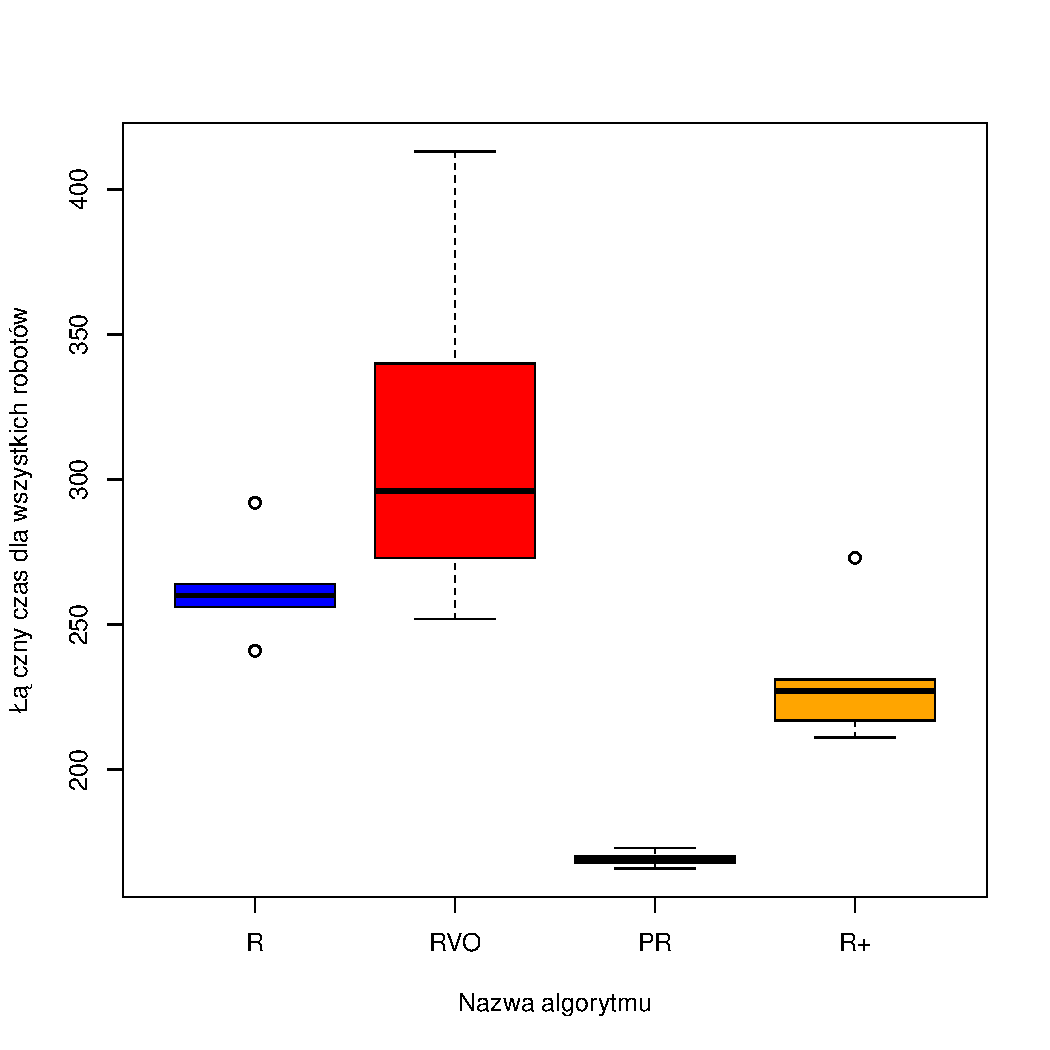
\includegraphics[page = 1, width=\textwidth]{img/Robots_Open_space.pdf}
%		\caption*{Ustawienie \textit{1-1}}
%	\end{subfigure}	
%	\begin{subfigure}[b]{0.49\textwidth}
%		\includegraphics[page = 2, width=\textwidth]{img/Robots_Open_space.pdf}
%		\caption*{Ustawienie \textit{1-2}}
%	\end{subfigure}
%\end{figure}

%\end{frame}





%\begin{figure}[!ht]
%	\centering
%	\begin{subfigure}[b]{0.49\textwidth}
%		\includegraphics[page = 1, width=\textwidth]{06_experimental_results/robot/img/Robots_Passage_through_the_door.pdf}
%		\caption*{Ustawienie \textit{1-H1}}	
%	\end{subfigure}
%	\begin{subfigure}[b]{0.49\textwidth}
%		\includegraphics[page = 2, width=\textwidth]{06_experimental_results/robot/img/Robots_Passage_through_the_door.pdf}
%		\caption*{Ustawienie \textit{1-H2}}	
%	\end{subfigure}
%	\caption{Wyniki eksperymentów z wykorzystaniem  rzeczywistych robotów  mapa \textit{przejście przez drzwi}.}
%	\label{fig:Robot_1_H1}
%\end{figure}

%\end{frame}


%\section{Wyniki eksperymentów symulacyjnych}
%\begin{frame}
%\frametitle{\secname}
%\framesubtitle{otwarta przestrzeń 1-2}
%
%
%
%\begin{figure}[!hb]
%	
%	%	\includemovie[autoplay,repeat]{2cm}{2cm}{mov/OtwartaPrzestrzenR1-2.mpg}
%	%	\includemovie[autoplay,repeat]{2cm}{2cm}{mov/OtwartaPrzestrzenRVO1-2.mpg}
%	%	\includemovie[autoplay,repeat]{2cm}{2cm}{mov/OtwartaPrzestrzenPR1-2.mpg}
%	%	\includemovie[autoplay,repeat]{2cm}{2cm}{mov/OtwartaPrzestrzenR+1-2.mpg}
%\end{figure}
%
%
%\end{frame}

%
%
%\section{Wnioski i kierunki rozwoju}
%\begin{frame}
%\frametitle{\secname}
%
%\begin{itemize}
%	\item Behawioralny i zdecentralizowany algorytm sterowania ruchem robotów mobilnych, oparty o zachowania inspirowane postępowaniem przemieszczających się osób, może być wykorzystany do bezpiecznego i skutecznego koordynowania ruchu grup robotów działających w dynamicznie zmiennych środowiskach.
%	\item Algorytm oparty o zasadach społecznych sprawdza się znacznie lepiej w skomplikowanych przestrzeniach niż metoda Reciprocal Velocity Obstacles.
%\end{itemize}
%
%\begin{figure}[!hb]
%	
%	\includemovie[autoplay,repeat]{2cm}{2cm}{mov/OtwartaPrzestrzenR1-2.mpg}
%	\includemovie[autoplay,repeat]{2cm}{2cm}{mov/OtwartaPrzestrzenRVO1-2.mpg}
%	\includemovie[autoplay,repeat]{2cm}{2cm}{mov/OtwartaPrzestrzenPR1-2.mpg}
%	\includemovie[autoplay,repeat]{2cm}{2cm}{mov/OtwartaPrzestrzenR+1-2.mpg}
%	
%\end{figure}
%
%\note{
%	Bezpieczna koordynacja ruchu rozumiana jest jako bezkolizyjne przemieszczanie się robotów.
%	
%	Skuteczność koordynacji rozumiana jest jako osiągnięcie postawionego przed robotami celu (przemieszczenie się od punktu startu do punktu docelowego) oraz nie powodowanie zakleszczeń. W pracy rozważono zestaw wybranych, najbardziej popularnych środowisk, w których potencjalnie może dochodzić do zakleszczeń na przykład w trakcie pokonywania: skrzyżowań, wąskich przejść, wąskich korytarzy czy mijanek.
%	
%}
%
%\end{frame}
%
%
%\section{Wnioski i kierunki rozwoju}
%\begin{frame}
%\frametitle{\secname}
%
%\begin{itemize}
%\item Wymuszenie ustępowania pierwszeństwa w wąskich traktach komunikacyjnych zwiększa jego przepustowość.
%
%\end{itemize}
%
%\begin{figure}[!hb]
%
%\includemovie[autoplay,repeat]{2cm}{2cm}{mov/PrzejsciePrzezDrzwiR1-H2.mpg}
%\includemovie[autoplay,repeat]{2cm}{2cm}{mov/PrzejsciePrzezDrzwiPF1-H2.mpg}
%\includemovie[autoplay,repeat]{2cm}{2cm}{mov/PrzejsciePrzezDrzwiR+1-H2.mpg}
%\includemovie[autoplay,repeat]{2cm}{2cm}{mov/PrzejsciePrzezDrzwiPF+1-H2.mpg}
%
%\end{figure}
%
%\end{frame}
%
%
%
%\section{Wnioski i kierunki rozwoju}
%\begin{frame}
%\frametitle{\secname}
%
%\begin{itemize}
%
%\item Zdefiniowanie stanów wychodzenie lub wchodzenia w zależności do obserwowanych czynników: np. powierzchnia pomieszczenia, liczba drzwi, gęstość robotów.
%
%\item Rozpowszechnienie informacji o bazowym współczynniku respektu -- wykorzystanie obserwowanej chwilowej prędkości robotów.
%
%\item Wyznaczenie pierwszeństwa poruszanie w oparciu o zasady obowiązujące w ruchu żeglugowym.
%\end{itemize}
%
%
%\note{Prezentowane wyniki pokazują, iż poprzez wprowadzając zasady pierwszeństwa, w drzwiach wydajność przemieszczenia się robotów poprawiła się. Oparty o zasady społeczne algorytm koordynacji sprawdza, się w skomplikowanych przestrzeniach znacznie lepiej, niż metoda referencyjna \emph{Reciprocal Velocity Obstacles}. 
%
%Dalsze pracę nad algorytmem koncentrować się będą, na zdefiniowaniu stanu wychodzenia lub wchodzenia w zależności od obserwowalnych czynników, np. powierzchni pomieszczeń, liczby ich drzwi, lub gęstości robotów znajdujących się w pomieszczeniu. 
%
%Wadą obecnej implementacji jest, z pewnością rozpowszechnianie informacji o bazowym współczynniku respektu każdego z robotów, który jest niezbędny do wyznaczania pierwszeństwa w sytuacjach "jeden na jeden". Rozwiązaniem tego problemu, może być wykorzystanie obserwowanej prędkości chwilowej każdego z robotów. 
%}
%
%\end{frame}
%
%
%
%\section*{Wnioski i kierunki rozwoju}
%\begin{frame}
%\frametitle{\secname}
%
%\begin{itemize}
%\item Zestaw prostych reaktywnych reguł jest dość dobrą metodą koordynacji ruch robotów w zatłoczonych środowiskach charakteryzującą się dużą dynamikę ruchu.
%
%\item Ilość potrzebnej do bezpiecznego wyminięcia się przestrzeni determinuje również zastosowana metoda koordynacji.
%\end{itemize}
%
%\note{Bazując na pozyskiwanych z otoczenia informacji możliwe jest stworzenie zdecentralizowanego algorytmu koordynującego ruch poszczególnych niezależnych jednostek mobilnych. W oparciu o dostarczone ze środowiska dane, algorytm jest wstanie reagować na dynamicznie zmieniającą się sytuację w jego najbliższym sąsiedztwie. Bazując wyłącznie na obserwacji środowiska, roboty są w stanie, bez konieczności wymiany komunikatów, koordynować swój ruch starając się przy tym stale podążać do celu.
%
%Testy potwierdziły również skuteczności działania mechanizmu rozwiązywania sytuacji konfliktowych (wzajemnych zakleszczeń).
%
%Brak centralnego punktu sterownia oraz zdecentralizowane podejmowanie decyzji czynią tak stworzony system wielorobotowy odpornym na awarię. 
%
%Testy w \textit{otwartej przestrzeni} wykazały, iż droga jaką muszą pokonać roboty znacznie różni się w zależności od cech, które posiadają poszczególne algorytmy. Roboty w metodzie \textit{PR} muszą ''nadkładać'' drogi, aby ustąpić pierwszeństwa zaś w~metodach bazujących na respekcie, (\textit{R} oraz \textit{R+}), roboty poruszają się mniej skomplikowanymi drogami.
%}
%
%\end{frame}
%
%
%
%\section*{Wnioski i kierunki rozwoju}
%\begin{frame}
%\frametitle{\secname}
%
%\begin{itemize}
%\item Uzależnienie stanu wychodzenie lub wchodzenia od obserwowanej sytuacji: np. powierzchnia pomieszczenia, liczba drzwi, gęstość robotów.
%
%\end{itemize}
%
%\note{Niekorzystny wpływ bazowego współczynnikiem respektu na pokonywaną drogę przez roboty.
%
%
%Przeprowadzone eksperymenty uwydatniły również niedoskonałości metody behawioralnej związanej z \textit{bazowym współczynnikiem respektu}. W eksperymencie \textit{otwarta przestrzeń skos} robot z powodu niskiego \textit{bazowego współczynnika respektu} musi ''nadkładać'' drogi w celu ominięcia robota o wyższym \textit{współczynniku respektu} (rozdział \ref{Wyniki_Otwarta_przestrzen_skos}). 
%
%
%W środowiskach bardziej skomplikowanych, jak  \textit{przejście przez drzwi}, lepiej radzą sobie metody, które wymuszają przepustowość traktu komunikacyjnego, nawet kosztem zatrzymania lub zmiany kierunku innych jednostek (rozdziały \ref{Wyniki_Przejscie_przez_drzwi} i \ref{Robot Przejście przez drzwi}). Podnosząc priorytet robotom, które wychodzą z pomieszczenia udrażniamy przejście i tym samym zwiększamy jego przepustowość.}
%
%\end{frame}


%Problem wzajemnego „przepychania się” robotów w wąskich przejściach. 


%
%
%
%
%
%
%\documentclass[notes]{beamer}       % print frame + notes
%%\documentclass[notes=only]{beamer}   % only notes
%%\documentclass{beamer}              % only frames
%
%
%%\setbeameroption{show notes on second screen=right} % Both
%
%% Give a slight yellow tint to the notes page
%\setbeamertemplate{note page}{\pagecolor{yellow!5}\insertnote}\usepackage{palatino}
%
%\usepackage[polish]{babel}
%\usepackage[utf8]{inputenc}
%\usepackage{lmodern}
%
%\usetheme{AGH}
%

%
%\begin{document}
%
%\titleframe[pl]
%
%\begin{frame}
%\frametitle{Zwykły slajd...}
%\framesubtitle{...z podtytułem...}
%    \begin{itemize}[<+-|alert@+>]
%        \item ...i zwykłą treścią.
%    \end{itemize}
%\note{Everything you want}
%\end{frame}
%
%
%
%\begin{frame}
%\frametitle{Inspiracja – zjawisko respektu}
%
%\begin{itemize}[<+-|alert@+>]
%	\item ...i zwykłą treścią.	
%\end{itemize}
%\end{frame}

%
%\section{Zwykły slajd... ala ma kota szsz}	
%\begin{frame}
%\frametitle{\secname}
%%\framesubtitle{...z podtytułem...}
%
%\begin{itemize}
%	\item Here are
%	\item some very boring bullets
%	\item about nothing.
%\end{itemize}
%
%\note[item]{Note that this slide is boring.}
%
%\note[item]{Observe that there are no actual bullets here.}
%
%\note[item]{Future work: add another bullet.}
%\end{frame}
%
%
%\section{Zwykły 2}	
%\begin{frame}
%\frametitle{\secname}
%%\framesubtitle{...z podtytułem...}
%
%\begin{itemize}
%\item Here are
%\item some very boring bullets
%\item about nothing.
%\end{itemize}
%
%\note[item]{Note that this slide is boring. 1233}
%\end{frame}
%
%\section{teee}
%\begin{frame}
%\frametitle{\secname}
%%\framesubtitle{...z podtytułem...}
%
%Jakis długi teskt a pod nim filmiki:fdgfdsfgdsfds fds 
%fdsf
%dsfdsf
%dsf
%dsf
%ds dfd
%
%Jakis  ubtt tejst
%
%\begin{itemize}
%\item znam robota
%\item nie wiem gdzie jest
%\end{itemize}
%
%
%\begin{figure}[!hb]
%
%\includemovie[autoplay,repeat]{3cm}{3cm}{mov/test2.mpg}
%\includemovie[autoplay,repeat]{3cm}{3cm}{mov/test3.mpg}
%\includemovie[autoplay,repeat]{3cm}{3cm}{mov/test4.mpg}
%\end{figure}
%
%\end{frame}

%
%
%\end{document}
